\section{第十六周数值分析实验}
\subsection{Jacobi和G-S迭代法}
\begin{ex}
设线性方程组
$$
\left\{\begin{array}{l}
	x_1+2 x_2-2 x_3=1, \\
	x_1+x_2+x_3=1, \\
	2 x_1+2 x_2+x_3=1 .
\end{array}\right.
$$

试编制程序, 列表给出前 10 个迭代向量, 并考察 $J a c o b i$ 和 $G-S$ 迭代法的收玫性.
\end{ex}
\lstinputlisting[language=matlab]{w16/q1.m}
\qa 
% Table generated by Excel2LaTeX from sheet 'Sheet1'
\begin{table}[H]
	\centering
	\caption{运行结果}
	\begin{tabular}{|c|ccccccccccc|}
		\hline
		$n$(Jacobi) & 0     & 1     & 2     & 3     & 4     & 5     & 6     & 7     & 8     & 9     & 10 \\
		\hline
		$x_1$    & 0     & 1     & 1     & -3    & -3    & -3    & -3    & -3    & -3    & -3    & -3 \\
		$x_2$   & 0     & 1     & -1    & 3     & 3     & 3     & 3     & 3     & 3     & 3     & 3 \\
		$x_3$    & 0     & 1     & -3    & 1     & 1     & 1     & 1     & 1     & 1     & 1     & 1 \\
		\hline\hline
		$n$(G-S) & 0     & 1     & 2     & 3     & 4     & 5     & 6     & 7     & 8     & 9     & 10 \\
		\hline
		$x_1$    & 0     & 1     & -1    & -11   & -43   & -131  & -355  & -899  & -2179 & -5123 & -11779 \\
		$x_2$    & 0     & 0     & 3     & 15    & 51    & 147   & 387   & 963   & 2307  & 5379  & 12291 \\
		$x_3$    & 0     & -1    & -3    & -7    & -15   & -31   & -63   & -127  & -255  & -511  & -1023 \\
		\hline
	\end{tabular}%
	\label{tab:addlabel-w16-1}%
\end{table}%


\subsection{SOR迭代法}
\begin{ex}
	用 $S O R$ 方法解线性方程组
	$$
	\left(\begin{array}{cccc}
		4 & -1 & -1 & -1 \\
		-1 & 4 & -1 & -1 \\
		-1 & -1 & 4 & -1 \\
		-1 & -1 & -1 & 4
	\end{array}\right)\left(\begin{array}{l}
		x_1 \\
		x_2 \\
		x_3 \\
		x_4
	\end{array}\right)=\left(\begin{array}{l}
		1 \\
		1 \\
		1 \\
		1
	\end{array}\right)
	$$
	
	初值取 $x^{(0)}=(0,0,0,0)^T$, 计算到 $\left\|x^{(k)}-x^{(k-1)}\right\|_{\infty}<10^{-8}$ 停止, 并绘制迭代步数 IT 关于松驰因子 $\omega$ (步长取 0.01$)$ 的图像.
\end{ex}
\lstinputlisting[language=matlab]{w16/q2.m}
\qa
 $\mathbf{x}=\left[0.308641974897860,0.308641979217244,0.308641971803977,0.308641977711201\right]^T.$
\begin{figure}[H]
	\centering
	\subfloat[$0.01\leq \omega\leq 1.99$]{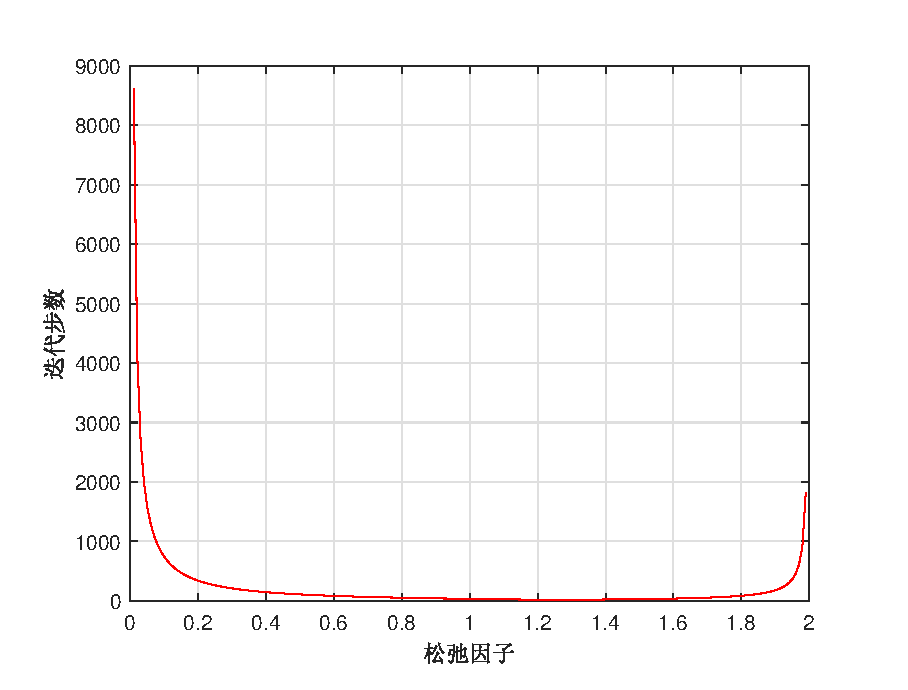
\includegraphics[width = 0.5\linewidth]{w16/q2-l.eps}}
	\hfill
	\subfloat[$0.40\leq \omega\leq 1.80$]{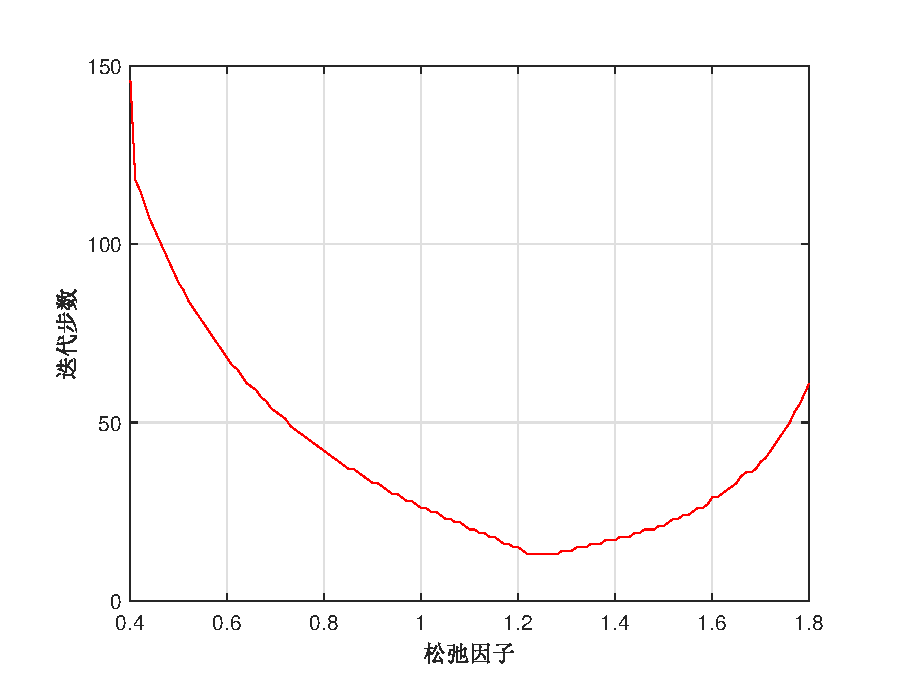
\includegraphics[width = 0.5\linewidth]{w16/q2-s.eps}}
	\caption{迭代步数}
\end{figure}
\subsection{选做题}
\begin{ex}
	已知 $50 \times 50$ 带状方程组, 设初始解向量为 $x^{(0)}=0.01$ ones $(50,1)$, 精度 $\varepsilon=10^{-14}$,试采用 Jacobi 迭代法和 $G-S$ 迭代法求解带状线性方程组满足精度要求的近似解.
	$$
	\left(\begin{array}{llllllll}
		12 & -2 & 1 & & & & & \\
		-2 & 12 & -2 & 1 & & & & \\
		1 & -2 & 12 & -2 & 1 & & & \\
		& 1 & -2 & 12 & -2 & 1 & & \\
		& & \ddots & \ddots & \ddots & \ddots & \ddots & \\
		& & & 1 & -2 & 12 & -2 & 1 \\
		& & & & 1 & -2 & 12 & -2 \\
		& & & & & 1 & -2 & 12
	\end{array}\right)\left(\begin{array}{c}
		x_1 \\
		x_2 \\
		x_3 \\
		x_4 \\
		\vdots \\
		x_{48} \\
		x_{49} \\
		x_{50}
	\end{array}\right)=\left(\begin{array}{c}
		5 \\
		5 \\
		5 \\
		5 \\
		\vdots \\
		5 \\
		5 \\
		5
	\end{array}\right)
	$$
\end{ex}
\lstinputlisting[language=matlab]{w16/q3.m}
\qa 
% Table generated by Excel2LaTeX from sheet 'Sheet1'
\begin{table}[H]
	\centering
	\caption{运行结果}
	\resizebox{1.1\columnwidth}{!}{
	\begin{tabular}{|cccccccc|}
		\hline
		$x_1$ & $x_2$ & $x_3$ & $x_4$ & $x_5$ & $x_6$ & $x_7$ & $x_8$ \\
		0.46379552381655 & 0.537284605199966 & 0.509022924601331 & 0.498221634436174 & 0.498941860239762 & 0.499985351248131 & 0.500088723890136 & 0.500015318846052 \\
		$x_{9}$ & $x_{10}$ & $x_{11}$ & $x_{12}$ & $x_{13}$ & $x_{14}$ & $x_{15}$ & $x_{16}$ \\
		0.499994793266975 & 0.499997856913468 & 0.500000108425199 & 0.500000201576687 & 0.500000022610945 & 0.499999986238572 & 0.499999995873979 & 0.500000000530294 \\
		$x_{17}$ & $x_{18}$ & $x_{19}$ & $x_{20}$ & $x_{21}$ & $x_{22}$ & $x_{23}$ & $x_{24}$ \\
		0.500000000439039 & 0.500000000023939 & 0.499999999966017 & 0.499999999992557 & 0.500000000001741 & 0.500000000000922 & 0.499999999999990 & 0.499999999999923 \\
		$x_{25}$ & $x_{26}$ & $x_{27}$ & $x_{28}$ & $x_{29}$ & $x_{30}$ & $x_{31}$ & $x_{32}$ \\
		0.499999999999998 & 0.499999999999987 & 0.499999999999921 & 0.500000000000001 & 0.500000000000915 & 0.500000000001741 & 0.499999999992558 & 0.499999999966019 \\
		$x_{33}$ & $x_{34}$ & $x_{35}$ & $x_{36}$ & $x_{37}$ & $x_{38}$ & $x_{39}$ & $x_{40}$ \\
		0.500000000023937 & 0.500000000439038 & 0.500000000530295 & 0.499999995873980 & 0.499999986238572 & 0.500000022610945 & 0.500000201576688 & 0.500000108425199 \\
		$x_{41}$ & $x_{42}$ & $x_{43}$ & $x_{44}$ & $x_{45}$ & $x_{46}$ & $x_{47}$ & $x_{48}$ \\
		0.499997856913467 & 0.499994793266975 & 0.500015318846052 & 0.500088723890136 & 0.499985351248131 & 0.498941860239762 & 0.498221634436174 & 0.509022924601331 \\
		$x_{49}$ & $x_{50}$ &       &       &       &       &       &  \\
		0.537284605199966 & 0.463795523816550 &       &       &       &       &       &  \\
		\hline
	\end{tabular}%
	}
	\label{tab:addlabel-w16-q3}%
\end{table}%

